\section{\lare{}\label{chap:lare}}
\subsection{Introduction\label{sec:lare_introduction}}
\lare{}, lightweight \ajax{} replacement engine, is built on top of PJAX and successor of PJAXR.
\\
The idea of \lare{} is to have the advantages of \ajax{} while trying to avoid it's disadvantages.
Introduced in Juli 2013, as an extended version of PJAX, it allows to replace multiple containers with a single request, instead of the limit to replace only one container.
Matching by the ID of an container it passes the duty to define which container should be replaced from the client-side to the server-side with setting the correct IDs.
Introducing the tags <lare-head> and <lare-body> it gives the ability to change meta tags or the page title in the <head> and replace containers inside the <body> with only one request.
\\
This means it achieves the same UX improvements and reduced load times as classical \ajax{}.
On the other hand \singlePageApplication{}s using \lare{} are easily crawlable by the most used crawlers without additional efforts.
It also uses the pushState function of the History interface to achieve full functionality of browsers incl. back- and forward buttons.
\lare{} is a generic solution for \singlePageApplication{}s and can be implemented in nearly every web application.

\noindent{}As shown in fig. \ref{fig:lare_replacements} only the needed parts of the content are replaced.
It shows the behaviour of \lare{} when clicking on the link to the second page of the P tags in the sample web application.
On the bottom left the \webPage{} is shown before the request.
On the top right the response, which consists of the container with the IDs tags\_headline and content, is displayed.
On the bottom right the result with the replaced containers is illustrated.
\newpage{}
\begin{figure}[H]
\centering
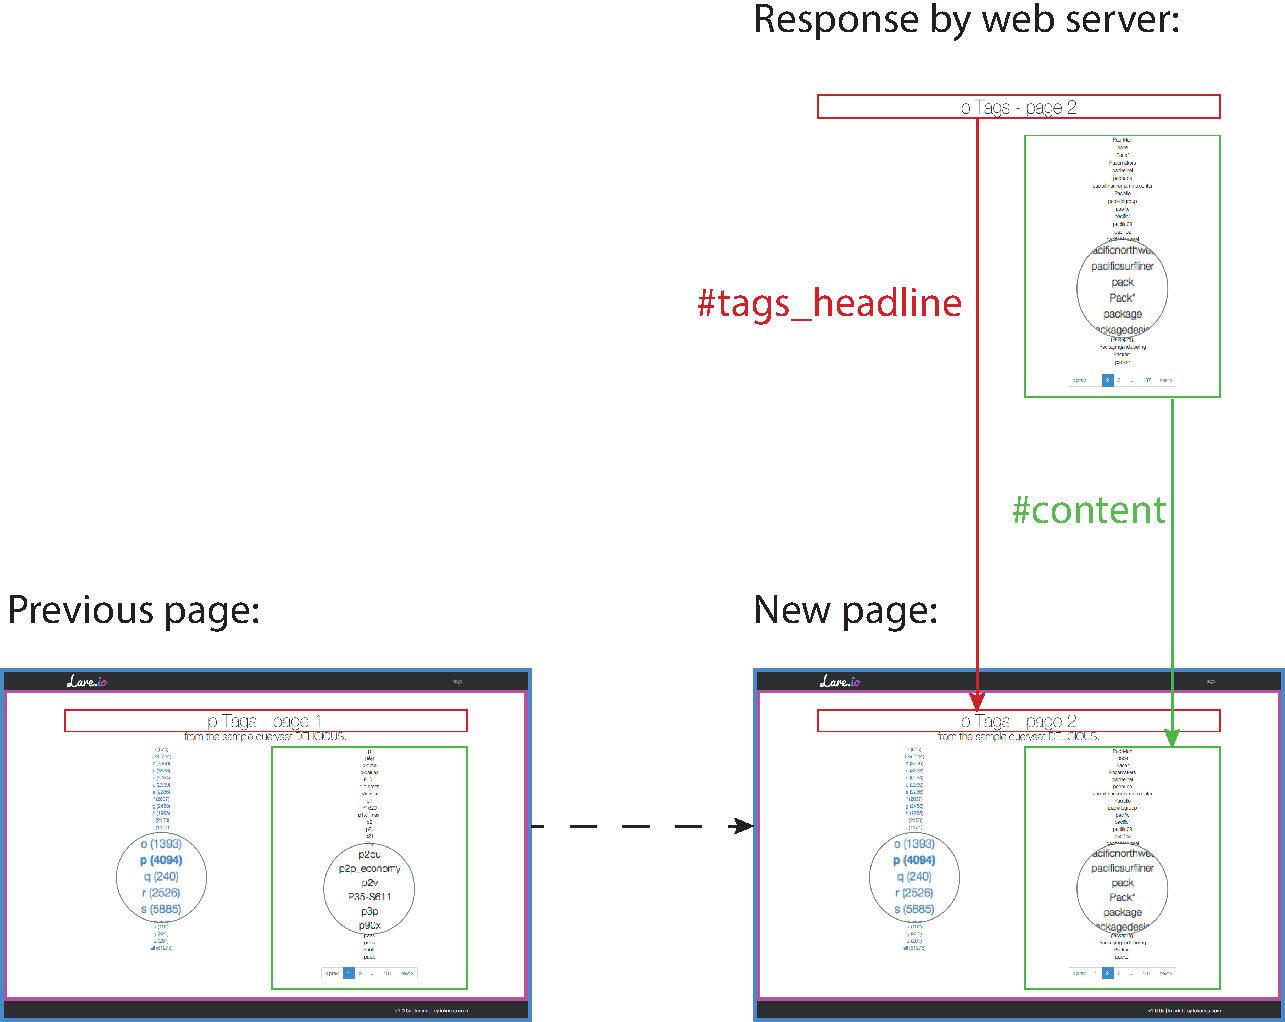
\includegraphics[width=14cm]{images/lare_replacements.pdf}
\caption[lare_replacements]{Content replacements by \lare{}}
\label{fig:lare_replacements}
\end{figure}

\subsection{Concept\label{sec:lare_concept}}

Every \singlePageApplication{} which uses \lare{} has a hierachical namespace structure.
Typically the namespace consists of up to four levels: A site ID, a page ID, a content ID and an inner-content ID.
In our sample web application namespaces like Lare.Tags.P1 are used.
\enquote{Lare} represents the site level, \enquote{Tags} the page and \enquote{P1} the content level.
Every level in the hierarchy has it's counterparts on the website as shown in figure \ref{fig:lare_html}.
There is no strict rule where exactly those containers have to be, but a container \emph{A} should not exist in another container \emph{B} if \emph{B} belongs to a namespace level above the one \emph{A} belongs to.
In this case when replacing \emph{B} with other content of the same level it could happen that \emph{A} could not be replaced anymore, because an object with this ID is not in the DOM anymore.
\\
After the \lare{} frontend is initialized it hijacks events like clicks on links and enriches the request with the current page's namespace.
A \lare{} backend plugged into the application analyzes the namespace of the requested page and the one sent in the request.
An earlier interpretation of the \lare{} namespaces like in a \webServer{} plugin for e.g. Apache\footnote{\url{http://httpd.apache.org/}} or Nginx\footnote{\url{http://nginx.org/}} is not possible, because the current request's namespace is set inside the application.
For every hierarchy level it checks if both namespaces match.
If on one level the namespaces don't match the containers according to this level will be responded to the request.
An optimized web application only grabs the data necessary for those containers and renders them afterwards.
The \lare{} frontend retrieves the response, replaces the containers at the website and updates the current namespace.

\begin{figure}[H]
\centering
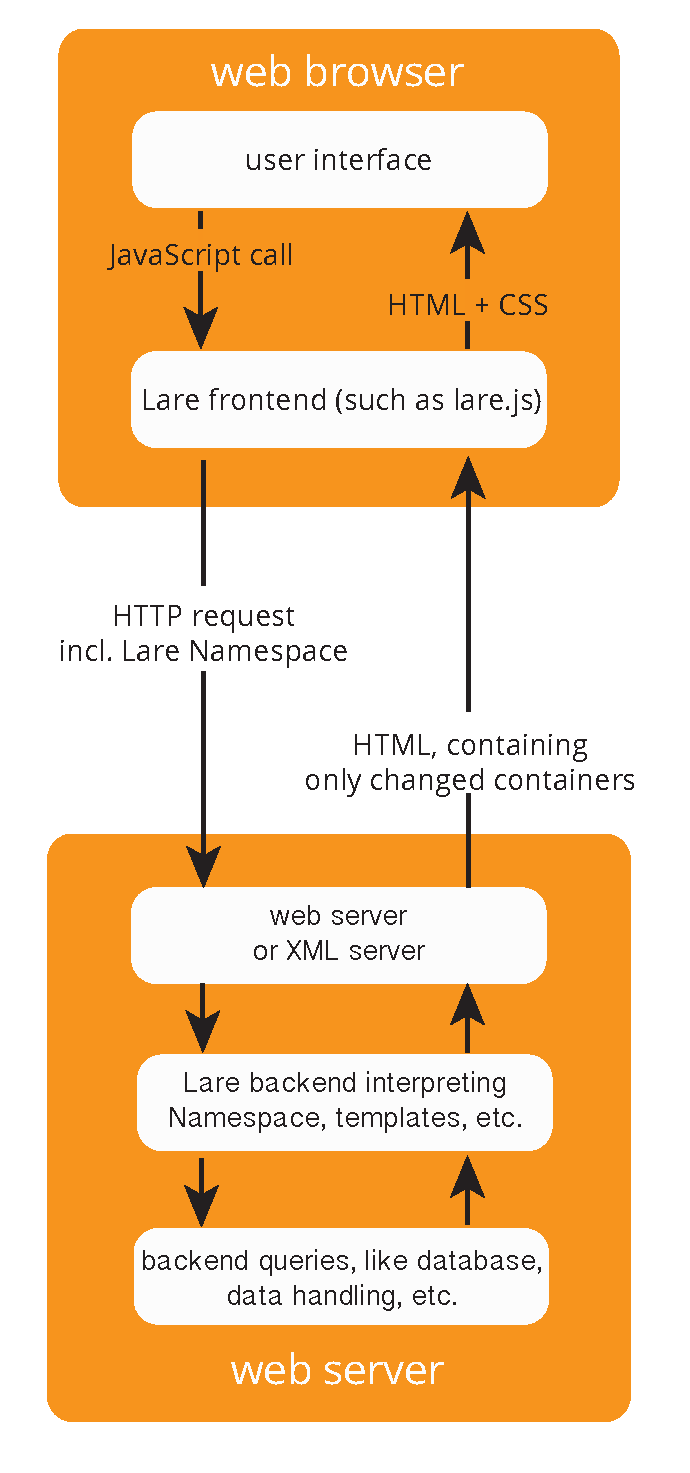
\includegraphics[height=15cm]{images/lare.pdf}
\caption[lare_components]{Components and communication diagram of \lare{}}
\label{fig:lare_components}
\end{figure}


\noindent{}As shown in fig. \ref{fig:lare_components} the rough structure of \lare{} is similar to normal \ajax{} requests shown in fig. \ref{fig:ajax_components}.
The \lare{} frontend, e.g. \lareJS{}, takes the place of the \ajax{} engine.
In addition to \ajax{}, \lare{} has a backend which helps to reduce server load and maps responses to the given namespace.
It can decide which backend queries such as database queries are necessary in the current request.
Also i should decide which templates are needed, as \lare{} responses have a different structure than normal HTML documents, which is presented later on.

\subsection{Realization\label{sec:lare_realization}}
To load a page, the first request is a normal \httpRequest{} followed by a JavaScript script initializing the \lare{} frontend module.
This delayed transfer of the frontend is not a problem, as the content can be rendered completely without it.
With this \lare{} follows the \hijax{} pattern, as it fully degrades for usage without JavaScript.
Further requests to the same host are then initiated by this module.
The \http{} header of these requests is extended by the namespace of the current website.
The web server using a \lare{} backend compares the namespace of the requested resource and the namespace in the \http{} header.
It then decides which data is needed to be gathered and which template should be used to render those.
\\
The content delivered by the \lare{} backend enriched web server is interpreted by the frontend module and replaces the related containers.
This replacement is implemented using the ID attribute.
Other methods identifying corresponding containers like e.g. X-Path are not as generic in it's position on the page as the ID.
When a container is injected into the Document Object Model(DOM) or the position within of a container is changed, the X-Path might not hit the correct container anymore.
For example the X-PATH //*[@id="page"]/div[2] will not hit anymore if the previous div gets deleted.
\\
Using the History API makes it then possible to update the URL like it would be made by normal requests.
This is realized with the use of the pushState method introduced in the History API.
Back- and forward-buttons and bookmarks in a browser will also work like on a normal request using this.
\\
Common \httpRequest{}s and \lare{} requests request the same URL, but on normal requests a full \webPage{} is responded, on \lare{} requests only the changed containers are.
Search engines and other crawlers are able to crawl every link they can find and request it as on common \webPage{}s without any deficit.

\subsubsection{\lare{} frontend\label{sec:lare_frontend}}

A \lare{} frontend has, as mentioned before, a few things to be implemented.
The first requirement is the ability to hijack page changes.
This can be implemented by replacing the default event listeners for anchor-tags.
A new event listener then has to implement an enrichment of the HTTP header by the namespace using the \enquote{HTTP-X-LARE} key.
On initial requests the current namespace should be served as an attribute at the <body> tag called data-lare-namespace.
\lare{} requests serve a new namespace as content of a tag <pjaxr-namespace>.
\\
The key feature of \lare{}, dynamic URL changes, have to be implemented after getting the response.
This should be done by using the pushState function.
\\
The biggest functionality of the \lare{} frontend is the replacement.
A response of a \lare{} request is divided into a <lare-head> tag, a <lare-body> tag and the <lare-namespace> tag.
Elements of the <lare-head> should be a new <title> tag and <meta> tags matching the new content. 
Additionally scripts or styles can be linked in this section when they are needed by the new content.
Tags in the head will be appended, if it's the title, it will be be replaced.
\\
The <lare-body> tag will contain the new content which should replace old one.
The id of every direct child of this tag will be searched on the current \webPage{} and will be replaced if found.
If the response consists of tags, not found on the current page they will be ignored.

\subsubsection{\lare{} backend\label{sec:lare_backend}}

A \lare{} backend should first interpret the \enquote{HTTP-X-LARE} item in the HTTP header.
Every layer of the namespace should have it's own name.
As a default naming convention the layers should have the names \emph{site}, \emph{page}, \emph{content}, \emph{inner\_content} from start to the end.
Per layer a variable should save the matching state.
Those variables have to be accessible by views and controllers to give them the possibility to decide which backend requests should be made and which templates should be used.

\subsubsection{\lare{} templating\label{sec:lare_templating}}

To avoid a lot of overhead when using \lare{} a specific templating system is recommended.
\\
A default template for initial requests could be like this:

\begin{minipage}[c]{0.95\linewidth}
\begin{lstlisting}[caption=\_\_base.html, label=lst:example_lare_base_template]
<!Doctype html>
<html>
<head>
  <title></title>
  <script src="lare.min.js"></script>
  ...
</head>
<body data-lare-namespace="{{lare_current_namespace}}">
  
    <div id="site">
      ...
      
      ...
    </div>
  
  
    <div id="additional_lare_includes"></div>
  
</body>
</html>
\end{lstlisting}
\end{minipage}
\\
The only specific code which is necessary for \lare{} to write is the \emph{data-lare-namespace} attribute at the body tag and the script in the head.
When using a template engine like Twig which can extend templates, \{\% block page \%\} represents a placeholder for where the page specific content will be rendered.
If only includes are available \{\% block page \%\} will be the position where the page specific content would be included.
\\
The \lare{} template could then be formed like this:

\begin{minipage}[c]{0.95\linewidth}
\begin{lstlisting}[caption=\_\_lare.html, label=lst:example_lare_template]
<lare-head>
  <title></title>
  ...
</lare-head>
<lare-body>
  
    
      
    
  
  
  
</lare-body>
<lare-namespace>{{lare_current_namespace}}</lare-namespace>
\end{lstlisting}
\end{minipage}
\\
The <lare-head> tag is the conterpart to the <head> tag, <lare-body> to <body>.
Instead of an attribute in the <lare-body> tag, the namespace will be delivered in the <lare-namespace> tag.
\\
The tags page in our sample web application consists of two templates.
On the one hand the character specific tags.html seen in listing \ref{lst:tags_template} which belongs to the third level namespace.
On the other hand there is \_\_tags\_base.html seen in listing \ref{lst:tags_base_template} which needs to get rendered only when entering the tags section and belongs to the second level namespace.

\begin{minipage}[c]{0.95\linewidth}
\begin{lstlisting}[caption=tags.html, label=lst:tags_template]


  <div id="content">
    ... // Tags list and pagination
  </div>


  <h1 id="tags_headline">
    {{ current_char }} Tags - page {{ current_page }}
  </h1>

\end{lstlisting}
\end{minipage}


\begin{minipage}[c]{0.95\linewidth}
\begin{lstlisting}[caption=\_\_tags\_base.html, label=lst:tags_base_template]


<div id="page">
  ...
  <h1 id="tags_headline">
    {{ current_char }} Tags - page {{ current_page }}
  </h1>
  ... // Character list
  
  ...
</div>

\end{lstlisting}
\end{minipage}

\noindent{}When e.g. navigating from the first page of P tags to the second page, the first two namespaces match, the third differ.
The third level belongs to \{\% block content \%\} in which the container with the id content is placed.
Additionally the container with the id tags\_headline is required to be replaced. As it is not a sibling of the content part it can be replaced in the additional\_lare\_includes block.
The response in this case would be this:

\begin{minipage}[c]{0.95\linewidth}
\begin{lstlisting}[caption=Example Lare Response, label=lst:lare_response]
<lare-body>
  <div id="content">
    ... // Tags list and Pagination
  </div>
  <div id="tags_headline">
    P Tags - page 2
  </div>
</lare-body>
<lare-namespace>Lare.Tags.P2</lare-namespace>
\end{lstlisting}
\end{minipage}

\noindent{}Both needed containers are rendered.
The content div is rendered, because it is defined in the content block and the tags\_headline div is defined inside the additional\_lare\_includes block.
\\
This block is intended to update content which is not inside the current level's container, in this case tags\_headline is inside the site level of the \enquote{Tags} namespace.
